
\documentclass{article}
\usepackage[spanish]{babel}
\usepackage[utf8]{inputenc}
\usepackage{amssymb, amsmath, amsbsy, wasysym}
\usepackage{multirow}
\usepackage{graphicx}
\usepackage{hyperref}
\title{Práctica 3\\Redes de computadoras}
\author{Emmanuel Peto Gutiérrez}
\begin{document}
\maketitle

\section{Pasos para realizar la práctica}

Se realizó un fork del repositorio del profesor para tenerlo en mi cuenta de git.

\url{https://gitlab.com/nehnemini/redes-2021-1/-/tree/master/lab3}

En la carpeta \texttt{lab3} se encuentra una página web. Tiene un formulario donde se pide un nombre de usuario y una contraseña.

La página se modificó, añadiendo código al archivo \texttt{style.css} y añadiendo una imágen (el escudo de la facultad de ciencias).

Para conectarse con AWS primero hay que iniciar la instancia creada en la práctica 2. Para esto hay que ir a la consola de AWS, entrar a la opción EC2, en el menú de la izquierda ir a \textit{Instancias/Instancias}, dar click en el id de la instancia y finalmente dar click en \texttt{Acciones/iniciar instancia.}

Una vez iniciada la instancia, me conecté desde mi equipo mediante el comando \texttt{ssh -i "practica2.pem" ubuntu@ec2-54-166-88-197.compute-1.amazonaws.com}

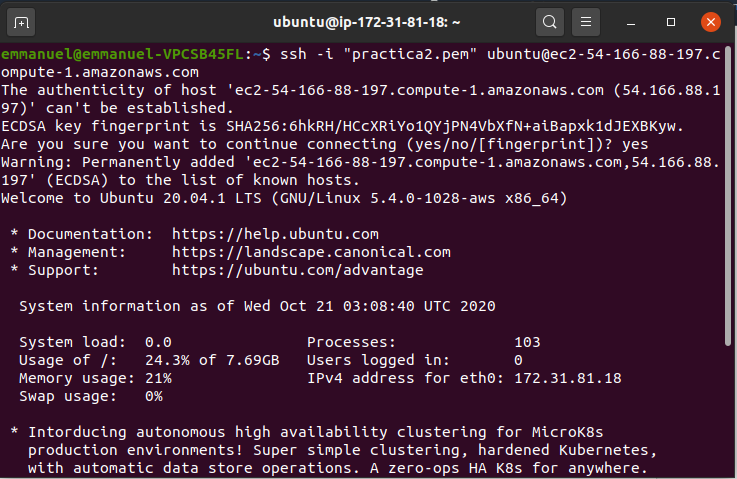
\includegraphics[width=\linewidth]{imagenes/paso1}

Luego, me cambié al directorio \texttt{/var/www/html/}. Al dar \texttt{ls} se muestra el archivo \textit{index.html} que se creó en la práctica 2.

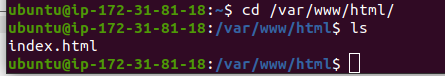
\includegraphics[width=\linewidth]{imagenes/paso2}

En este directorio cloné el repositorio \texttt{redes-2021-1}. Si se ejecuta el comando \texttt{ls} se debe mostrar la carpeta.

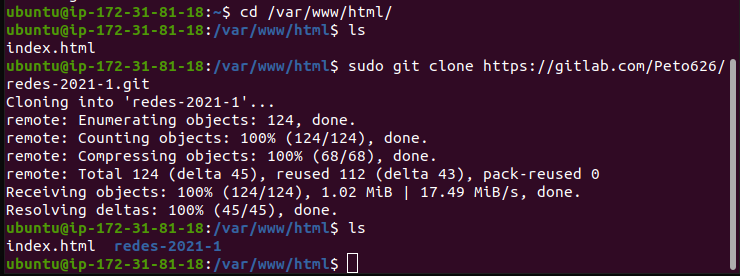
\includegraphics[width=\linewidth]{imagenes/paso3}

Hay que cambiar de dirección a \texttt{/etc/apache2/}. De aquí hay que entrar a \texttt{sites-available}. Se copia el archivo \texttt{000-default.conf} con el nuevo nombre \texttt{redesfc.conf}. El archivo recién copiado se abre con un editor de texto (\texttt{vi} en este caso).

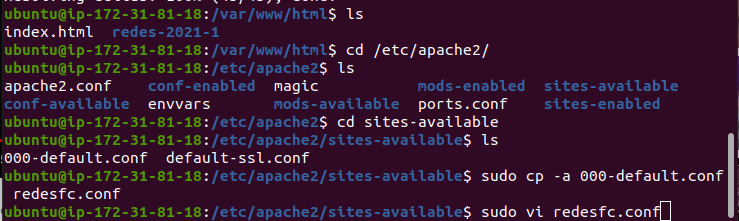
\includegraphics[width=\linewidth]{imagenes/paso4}

En la sección \texttt{DocumentRoot} se debe poner la dirección completa de la página web que se desea desplegar (debe haber un archivo \textit{index.html}). En este caso es \texttt{/var/www/html/redes-2021-1/lab3/codigo\_ejemplo}. Hay que guardar los cambios en el archivo y salir (\texttt{:x} en \texttt{vi}).

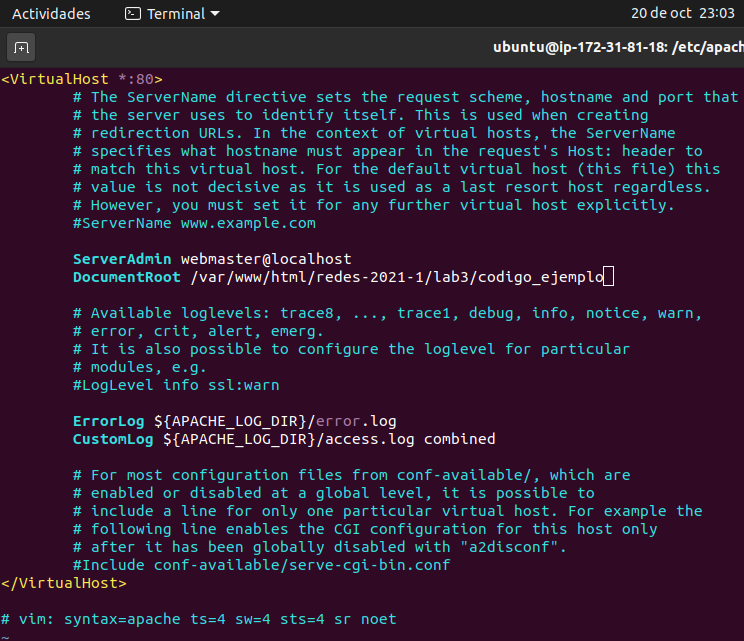
\includegraphics[width=\linewidth]{imagenes/paso5}

Hay que regresar al directorio \texttt{/var/www/html}. Actualmente, todos los cambios sólo pueden ser realizados por el administrador, así que hay que cambiar los permisos de la carpeta \texttt{redes-2021-1} para que el usuario \texttt{ubuntu:ubuntu} pueda hacer modificaciones. Claramente en otra situación el usuario puede tener otro nombre, pero en esta práctica es así. Para cambiar los permisos se ejecuta el comando \texttt{sudo chown -R ubuntu:ubuntu redes-2021-1/}

Una vez hecho esto, se debe deshabilitar el sitio de la práctica anterior (archivo \texttt{000-default.conf}) y habilitar el sitio de esta práctica (archivo \texttt{redesfc.conf}). Se ejecutan los comandos: \texttt{sudo a2dissite 000-default.conf} y \texttt{sudo a2ensite redesfc.conf}.

Luego, para aplicar los cambios, hay que reiniciar el servidor apache con el comando \texttt{sudo systemctl restart apache2.service}.

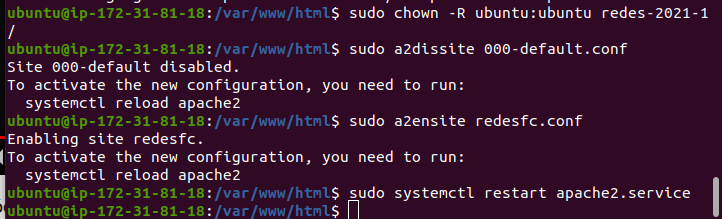
\includegraphics[width=\linewidth]{imagenes/paso6}

Se puede comprobar que la página que se muestra ahora es la de esta práctica, poniendo la dirección IP pública que provee AWS en un navegador.

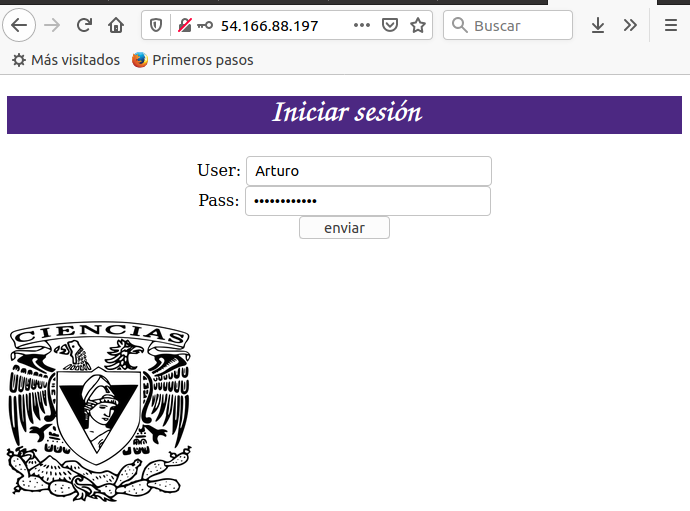
\includegraphics[width=\linewidth]{imagenes/paso7}

Si se coloca la IP seguida de un directorio se va a mostrar el contenido. En este caso, se está mostrando el contenido de \textit{images}. Para que no se muestre el contenido de los directorios hay que cambiar el archivo \texttt{redesfc.conf}.

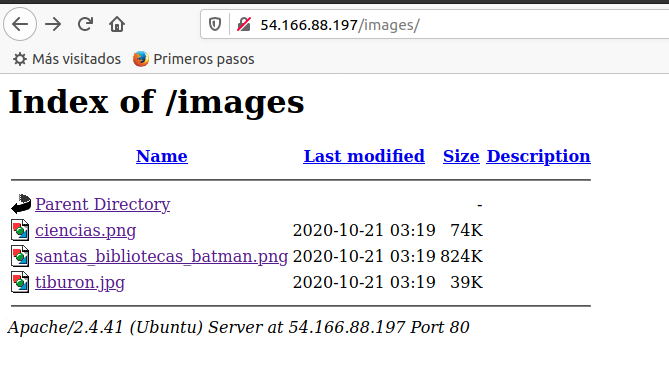
\includegraphics[width=\linewidth]{imagenes/paso8}

En la dirección \texttt{/etc/apache2/sites-available} se encuentra el archivo \texttt{redesfc.conf}, hay que abrirlo con \texttt{vi}. Para que no indexe el contenido hay que colocar el siguiente texto en el archivo:

\begin{verbatim}
<Directory /var/www/html/redes-2021-1/lab3/codigo_ejemplo>
    Options -Indexes
</Directory>
\end{verbatim}

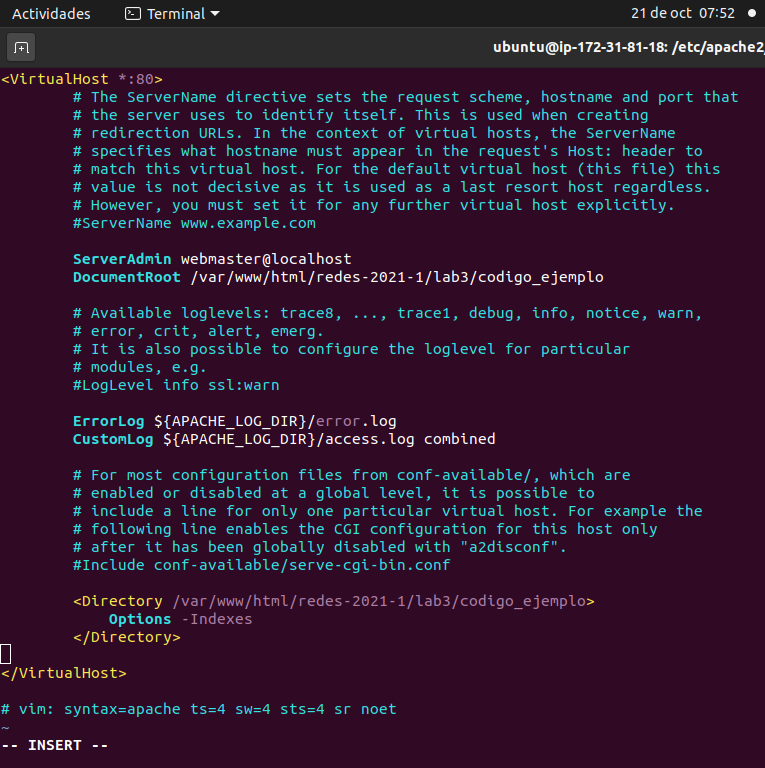
\includegraphics[width=\linewidth]{imagenes/paso9}

Para que se apliquen los cambios hay que reiniciar apache con \texttt{sudo systemctl restart apache2.service} (en la misma dirección en la que está \texttt{redesfc.conf}).

Ahora, si se intenta acceder a un directorio desde un navegador se mostrará un mensaje diciendo que no tengo permiso de acceder a ese recurso.

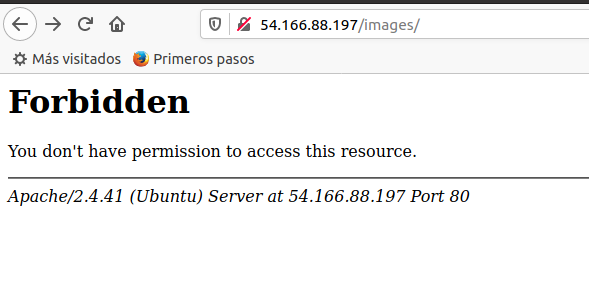
\includegraphics[width=\linewidth]{imagenes/paso10}

En la carpeta \texttt{cgi-bin} del código ejemplo se encuentra un script en Python que sirve para manejar los datos de entrada (usuario y contraseña). Hay que configurar el servidor para que ejecute el script. Para eso, en el directorio \texttt{/etc/apache2/sites-available}, hay que ejecutar el comando \texttt{sudo a2enmod cgid}. Para aplicar los cambios hay que reiniciar el servicio con \texttt{sudo systemctl restart apache2}.

Después, hay que abrir otra vez el archivo \texttt{redesfc.conf} y colocar las siguientes líneas:

\begin{verbatim}
ScriptAlias /cgi-bin/ /var/www/html/redes-2021-1/lab3/codigo_ejemplo/cgi-bin/

<IfModule cgid-module>
    <Directory /var/www/html/redes-2021-1/lab3/codigo_ejemplo/cgi-bin/>
        Options -Indexes
        Options +ExecCGI
        AddHandler cgi-script .py
    </Directory>
</IfModule>
\end{verbatim}

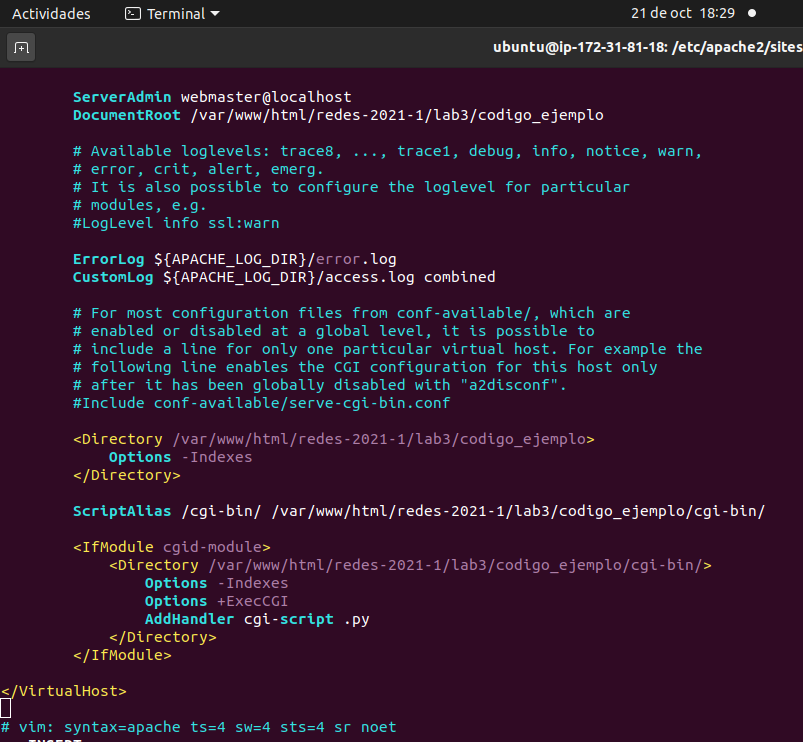
\includegraphics[width=\linewidth]{imagenes/paso11}

Una vez más, hay que aplicar los cambios con \texttt{sudo systemctl restart apache2.service}.

Para ver el tráfico entre mi computadora y la página que se acaba de crear se utiliza wireshark. Se coloca el filtro \texttt{ip.addr==54.166.88.197 and http}, que es la dirección de la página web y el protocolo que se desea filtrar.

Se coloca información de usuario y contraseña en el formulario y se da click a enviar, lo cual dará el siguiente resultado.

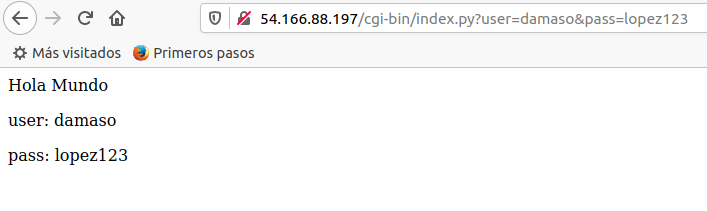
\includegraphics[width=\linewidth]{imagenes/paso12}

Y el tráfico en wireshark es el siguiente.

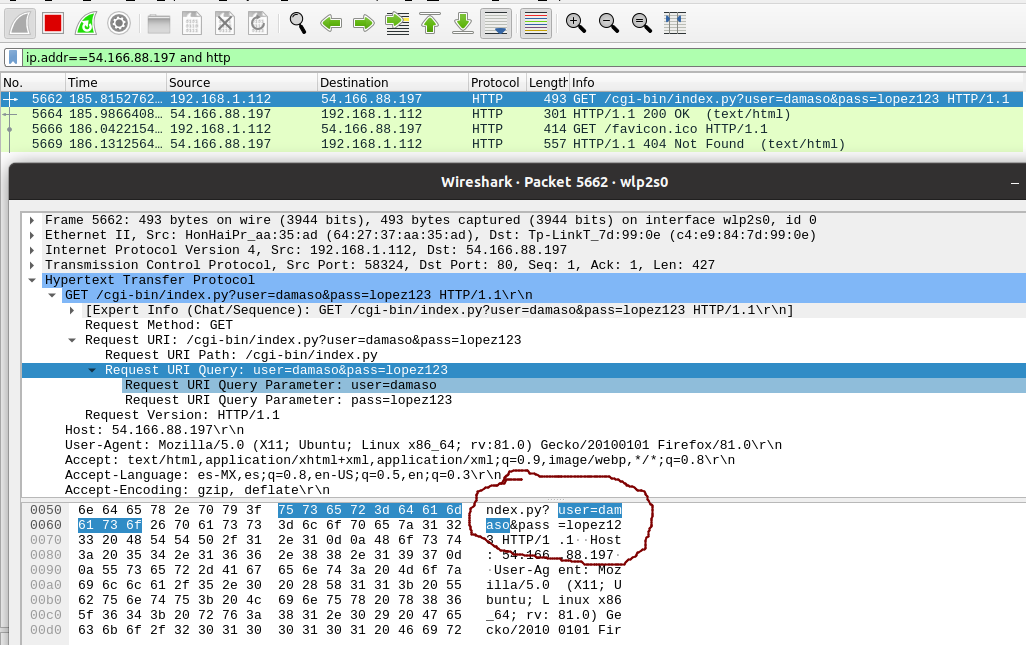
\includegraphics[width=\linewidth]{imagenes/paso13}

Como se notará, el resultado se envía mediante la url y es texto plano; es decir, no está cifrado.

Se procede a modificar el archivo \texttt{index.html} que se encuentra en el directorio \texttt{/var/www/html/redes-2021-1/lab3/codigo\_ejemplo}. En la acción del formulario ahora se va a usar el método \texttt{post} (antes se usaba el \texttt{get}); sólo hay que comentar una línea y quitarle el comentario a la otra.

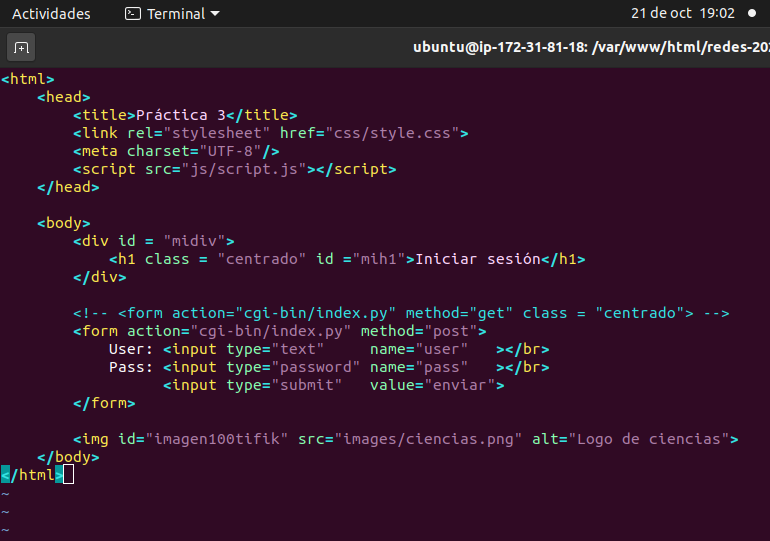
\includegraphics[width=\linewidth]{imagenes/paso14}

Otra vez hay que enviar los datos en el formulario. Ahora los datos de usuario y contraseña ya no se muestran en la url.

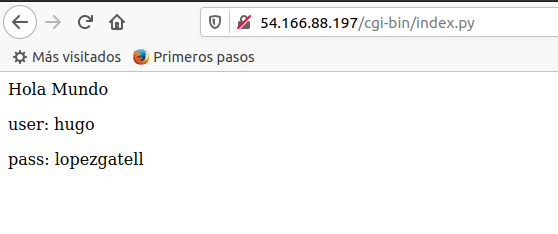
\includegraphics[width=\linewidth]{imagenes/paso15}

El tráfico generado por wireshark es el siguiente.

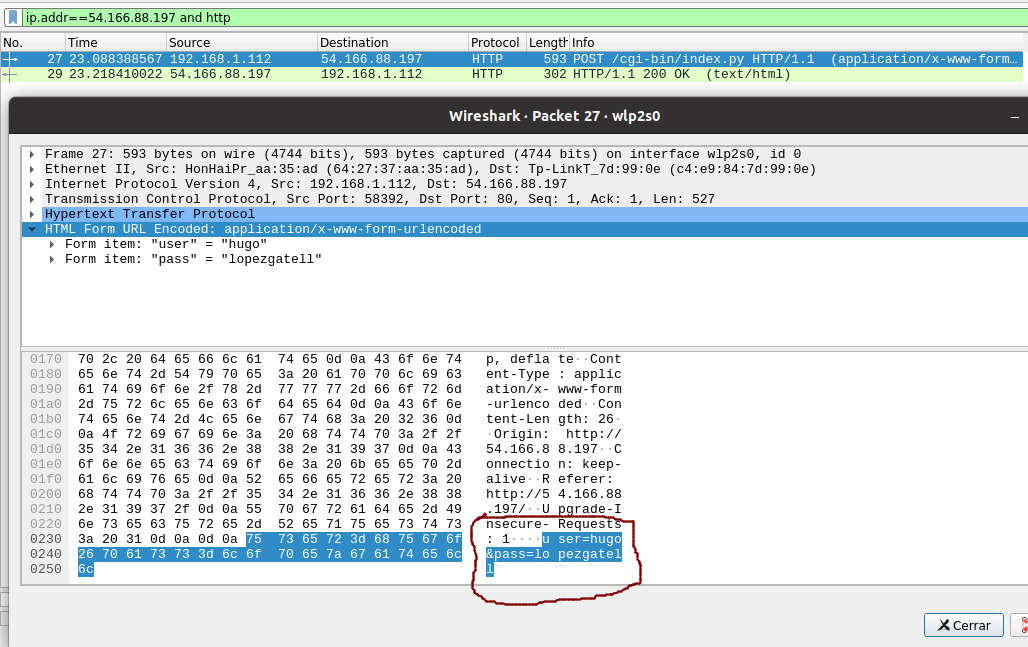
\includegraphics[width=\linewidth]{imagenes/paso16}

Como se nota, el nombre de usuario y contraseña se envían en texto plano de todas formas con el método \texttt{post}.

\section{Cuestionario}

\textbf{1. Menciona con tus propias palabras las ventajas que tiene centralizar el código fuente con git sin trabajar directamente en el servidor.}

La primera ventaja notada es que, en nuestras computadoras, podemos usar el editor de textos que queramos, mientras que en un servidor se debe trabajar en la terminal; también cambiar de un directorio a otro es más fácil en nuestras computadoras.

Al usar git es más fácil trabajar en equipo, pues se pueden crear ramas, tener control de versiones y notificar errores. Una vez terminado un proyecto, después de hacer pruebas, se puede clonar al servidor.\\

\textbf{2. ¿Para qué se usa la directiva} \texttt{Options -Indexes}?

Se usa para desindexar las carpetas y archivos de una aplicación web montada en un servidor. Así, las carpetas ya no son visibles para las personas que accedan a la página desde un navegador.\\

\textbf{3. Menciona algún concepto que no te haya quedado del todo claro (opcional).}

Sobre ``Apache'' (aunque no es un concepto): no entiendí por qué no se puede abrir una página web en el servidor sin haber instalado Apache en éste.

Por otra parte, no pude ejecutar el script de Python cuando probé el formulario en mi computadora.\\

\textbf{4. Liga del repositorio GitLab del repositorio con tus cambios.}

\url{https://gitlab.com/Peto626/redes-2021-1}\\

\textbf{5. Captura de pantalla del tráfico http (no seguro) con wireshark, marcando en dónde se envía la información en claro, tanto para el método GET como para el método POST.}

En la región encerrada se encuentra la información de usuario y contraseña enviada en el mensaje. La primera imagen es la del método GET y la segunda la de POST.

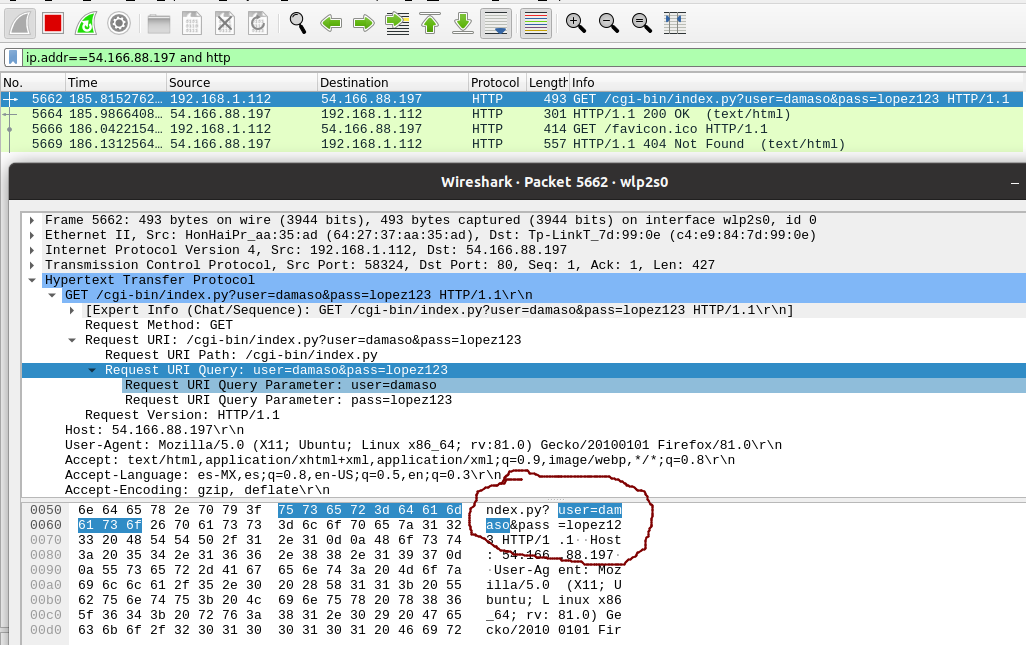
\includegraphics[width=\linewidth]{imagenes/paso13}

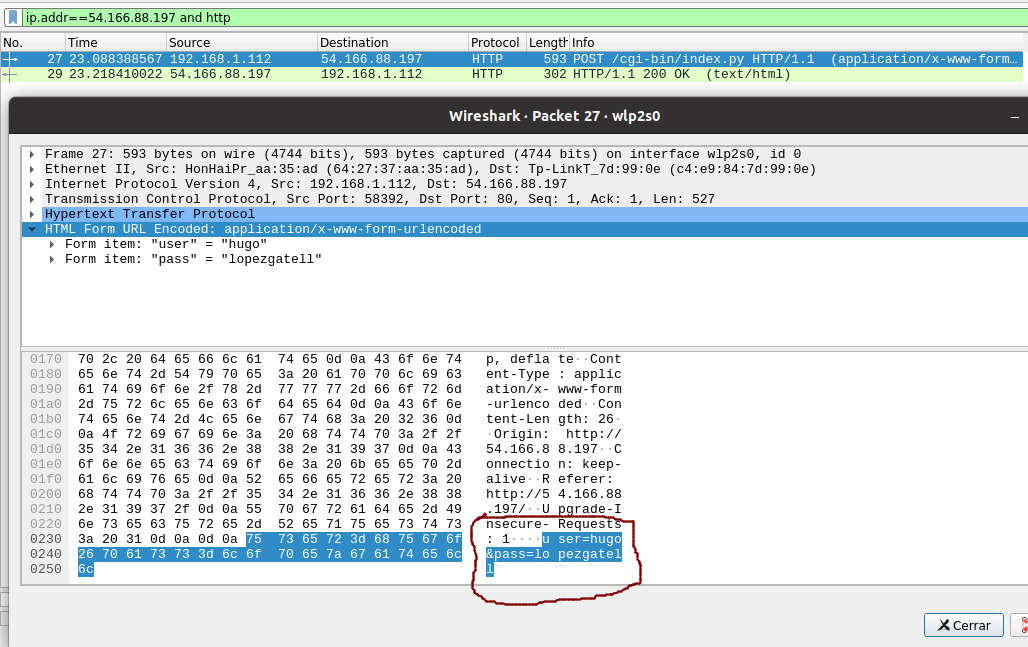
\includegraphics[width=\linewidth]{imagenes/paso16}

\textbf{6. ¿Cuál es la diferencia que se aprecia en Wireshark entre los mensajes que en donde se usó el método GET y los mensajes en donde se usa el método POST?, ¿cuál es la diferencia que se nota en el navegador web cuando se usa cada uno de estos métodos?}

En wireshark:\\En el método GET los datos aparecen en la sección de HTTP. Aquí se observa un \texttt{Request URI Path}, que es donde se encuentra el script de Python; también se ve un \texttt{Request URI Query} que es donde están los datos de \texttt{user} y \texttt{pass}, que en este caso son \texttt{damaso} y \texttt{lopez123}.

En el método POST los datos están contenidos en una sección llamada \texttt{HTML Form URL Encoded}. Los datos son items del formulario, donde las llaves son ``user'' y ``pass'' mientras que los valores asociados a esas llaves son ``hugo'' y ``lopezgatell''.

En el navegador:\\
Para el método GET, los datos de usuario y contraseña aparecen en la URL de la página, después de la ruta del script, como \texttt{user=damaso\&pass=lopez123}.

En cambio, en el método POST, no aparecen los datos de usuario y contraseña en la URL, sino que solo aparece la ruta del script: \texttt{/cgi-bin/index.py}.

\end{document}

